\chapter{\IfLanguageName{dutch}{Toestellen}{Devices}}
\label{ch:vergelijking}
Voor de proof of concept werd er goed nagedacht welke locatiebepaling-technologieën gebruikt kunnen worden. Het moet niet enkel functioneren in ideale omstandigheden, maar ook in ongunstige. Er moet ook voldaan worden aan de volgende vereisten:
\begin{itemize}
    \item Mogelijkheid tot het bepalen van de locatie;
    \item Mogelijkheid tot het delen van de locatie via sms;
    \item Mogelijkheheid tot het delen van de locatie via roaming;
    \item Mogelijkheid om te werken op batterij;
    \item Mogelijkheid tot waterdichtheid;
    \item Zo goedkoop mogelijk blijven.
\end{itemize}
Naast deze eisen moet de batterijduur zo lang mogelijk meegaan en de locatiebepaling moet zo accuraat mogelijk zijn.
\newline
Er is bewust gekozen om geen smarthphones te gebruiken. Eerst en vooral hebben smartphones een hoog batterijverbruik omdat er de hele tijd een besturingssyteem actief is. Hiernaast zijn GPS chips die gebruikt worden in smarthphones vaak inaccuraat.
\newline
\subsection{\IfLanguageName{dutch}{Raspberry Pi}{Raspberry Pi}}
Er bestaan verschillende veries van de Raspberry Pi. De versies die in aanmerking komen kunnen teruggevonden worden in tabel \ref{tab:rpimodellen}
\begin{table}[]
	\begin{tabular}{ll}
		\textbf{Model}                  & \textbf{Prijs (euro)} \\
		Raspberry Pi 4 Model B & 39.95        \\
		Raspberry Pi 3 B+      & 39.95        \\
		Raspberry Pi 3 B       & 37.95        \\
		Raspberry Pi 3 A+      & 26.80       
	\end{tabular}
\caption{Prijsvergelijking modellen Raspberry Pi. De prijzen zijn geraadpleegd op \url{https://www.raspberrypi.org/products}}
\label{tab:rpimodellen}
\end{table}
\newline
Naast de Raspberry Pi zijn er nog componenten nodig (zie tabel:\ref{tab:rpi}).
\begin{table}[]
	\begin{tabular}{llll}
		\textbf{Component}           & \textbf{Prijs (euro)} & \textbf{Doel}                                                                & Link                                                                                                                                                                                                                             \\
		\href{https://www.raspberrypi.org/products}{Raspberry Pi 3A+}    & 26.80        & Het hoofd toestel, draait een besturingssysteem en voert alles aan. & https://www.raspberrypi.org/products                                                                                                                                                                                             \\
		\href{https://www.bol.com/nl/p/ philips-sd-kaart-8gb-sd-card-class-4/9200000023935849/?country=BE\&Referrer=ADVNLPPcefd2c00d536683c00927aff17000051123\& utm\_source=51123\&utm\_medium=Affiliates\&utm\_campaign=CPS\&utm\_content=txl}{SD-kaart (min. 8GB)} & 9.99         & Hierop wordt het besturingssysteem en het script opgeslagen.        & https://www.bol.com/nl/p/ philips-sd-kaart-8gb-sd-card-class-4/9200000023935849/?country=BE\&Referrer=ADVNLPPcefd2c00d536683c00927aff17000051123\& utm\_source=51123\&utm\_medium=Affiliates\&utm\_campaign=CPS\&utm\_content=txl \\
		\href{https://www.robotshop.com/eu/ en/gsm-gprsgnssbluetooth-hat-raspberry-pi.html}{GSM HAT}             & 46.61        & Dit zorgt voor online communicatie om de data door te sturen.       & https://www.robotshop.com/eu/ en/gsm-gprsgnssbluetooth-hat-raspberry-pi.html                                                                                                                                                     \\
		\href{https://www.sossolutions.nl/1566-usb-battery-pack-for-raspberry-pi-10000mah-2-x-5v-outputs?gclid=CjwKCAjwvZv0BRA8EiwAD9T2VfLwMiBk7S2IyG0X13mIPVppguIaRPsgBf2mtAYpxLGU7K8PmdalmRoCbZgQAvD\_BwE}{5V} Battery          & 54.95        & Hierdoor kan de proof of concept draadloos werken.                  & https://www.sossolutions.nl/1566-usb-battery-pack-for-raspberry-pi-10000mah-2-x-5v-outputs?gclid=CjwKCAjwvZv0BRA8EiwAD9T2VfLwMiBk7S2IyG0X13mIPVppguIaRPsgBf2mtAYpxLGU7K8PmdalmRoCbZgQAvD\_BwE                                    \\
		\href{https://www.sossolutions.nl/raspberry-pi-gps-hat?gclid=CjwKCAjwvZv0BRA8EiwAD9T2VZeOJ8Gh0lykmCo9hwT2Zn5j8bvYHn\_mQX2lXPTCSkvUFwH6F3qQexoCutYQAvD\_BwE}{GPS HAT}             & 39.95        & Een meer accurate locatiebepaling in vergelijking met AGPS.         & https://www.sossolutions.nl/raspberry-pi-gps-hat?gclid=CjwKCAjwvZv0BRA8EiwAD9T2VZeOJ8Gh0lykmCo9hwT2Zn5j8bvYHn\_mQX2lXPTCSkvUFwH6F3qQexoCutYQAvD\_BwE                                                                             \\
		Totale kost:        & \textbf{178.30}        &                                                                     &                                                                                                                                                                                                                                 
	\end{tabular}
\caption{Prijs opstelling Raspberry Pi}
\label{tab:rpi}
\end{table}

\subsection{\IfLanguageName{dutch}{Arduino}{Arduino}}
Er kan eveneens gebruik gemaakt worden van een Arduino. Arduino heeft een module die geprogrammeerd kan worden om te voldoen aan alle eisen, namelijk de MKR 1400 GSM module. (Zie figuur: \ref{fig:mkr1400}) Er zijn uiteraard nog componenten nodig (zie tabel: \ref{tab:arduino}).
\begin{table}[]
	\begin{tabular}{llll}
		\textbf{Component}         & \textbf{Prijs (euro)} & \textbf{Doel}                                                               & Link                                                                     \\
		\href{https://store.arduino.cc/arduino-mkr-gsm-1400-1415}{MKR GSM}           & 80.35        & Dit component runt het script en stuurt de andere componenten aan. & https://store.arduino.cc/arduino-mkr-gsm-1400-1415                       \\
		\href{https://store.arduino.cc/arduino-mkr-gps-shield}{MKR GPS Shield}    & 41.75        & Een meer accurate lokatiebepaling in vergelijking met GPRS.        & https://store.arduino.cc/arduino-mkr-gps-shield                          \\
		\href{https://www.kiwi-electronics.nl/lithium-ion-polymer-battery-3-7v-2500mAh}{LiPo 3.7V 2500mAh} & 25.90        & Dit zorgt ervoor dat het MKR board draadloos kan werken.           & https://www.kiwi-electronics.nl/lithium-ion-polymer-battery-3-7v-2500mAh \\
		Totale kost:      & \textbf{148.00}       &                                                                    &                                                                         
	\end{tabular}
\caption{Prijs opstelling Arduino}
\label{tab:arduino}
\end{table}

\begin{figure}
    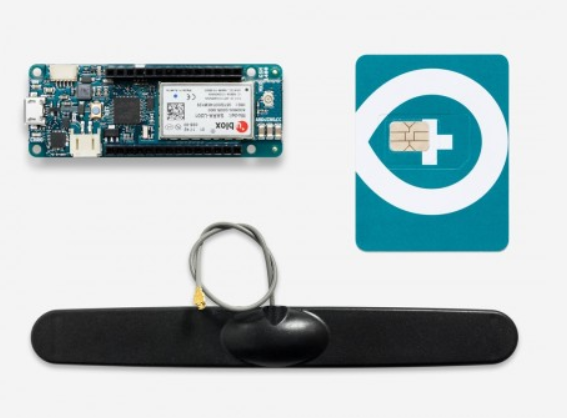
\includegraphics[width=\textwidth,height=\textheight,keepaspectratio]{mkr1400gsm.png}
    %https://store.arduino.cc/arduino-sim-mkr-gsm-1400-cellular-kit-1417?fbclid=IwAR0kJk6t6PVON-YakV_EiSOnb5y2RgBRQW0c6pVmpRw-hJlPRHO99qDdjSA
    \caption{\href{https://store.arduino.cc/arduino-sim-mkr-gsm-1400-cellular-kit-1417?fbclid=IwAR0kJk6t6PVON-YakV_EiSOnb5y2RgBRQW0c6pVmpRw-hJlPRHO99qDdjSA}{Arduino MKR 1400 GSM module}}
    \label{fig:mkr1400}
\end{figure}